\ExplSyntaxOn
\sys_gset_rand_seed:n {42}
\ExplSyntaxOff
\DocumentMetadata{pdfstandard=A-3a,pdfstandard=X-5,pdfstandard=UA-1,lang=en-US,pdfversion=1.7,testphase={phase-I,firstaid,title,graphic}}

\PassOptionsToPackage{scaled=0.85}{roboto-mono}
\documentclass[
	english,
	ruledheaders=section,
	class=report,
	thesis={type=bachelor},
	accentcolor=9c,
	custommargins=true,
	marginpar=false,
	parskip=half-,
	fontsize=11pt,
    listof=totoc
]{tudapub}

\usepackage[export]{adjustbox}

\usepackage[german, main=english]{babel}

\usepackage{microtype}

\usepackage{unicode-math}

\newcommand{\todo}[2][]{{\color{red} TODO: {#2}}}

\definecolor{mygreen}{RGB}{38,162,105}

\usepackage[acronym]{glossaries-extra}

\setabbreviationstyle[acronym]{long-short}

\renewcommand{\glsxtrtitleopts}{}

\newignoredglossary{ignored}

\makeglossaries

\newglossaryentry{simple algorithm}
{
    type={ignored},
    name=simple algorithm,
    description={Our algorithm without batching and without an AVL tree}
}

\newglossaryentry{simple ID}
{
    type={ignored},
    name=simple ID,
    description={The ID for our simple algorithm}  
}

\newglossaryentry{batching ID}
{
    type={ignored},
    name=batching ID,
    description={The ID for our batching algorithm}
}

\newglossaryentry{batching algorithm}
{
    type={ignored},
    name=batching algorithm,
    description={Our algorithm with batching but without an AVL tree}
}

\newglossaryentry{simple AVL algorithm}
{
    type={ignored},
    name=simple AVL algorithm,
    description={Our algorithm without batching but with an AVL tree}
}

\newglossaryentry{batching AVL algorithm}
{
    type={ignored},
    name=batching AVL algorithm,
    description={Our algorithm with batching and with an AVL tree}
}

\newacronym{crdt}{CRDT}{conflict-free replicated data type}
\newacronym{ot}{OT}{operational transformation}
\newacronym{oo}{OO}{Object-oriented}
\newacronym{fp}{FP}{Functional programming}
\newacronym{p2p}{P2P}{peer-to-peer}
\newacronym{dtn}{DTN}{delay tolerant network}
\newacronym{rdt}{RDT}{replicated data type}
\newacronym{woot}{WOOT}{WithOut Operational Transforms}
\newacronym{rga}{RGA}{Replicated Growable Array}
\newacronym{yata}{YATA}{Yet Another Transformation Approach}
\newacronym{manet}{MANET}{mobile ad hoc network}

\usepackage{fancyvrb}
\fvset{vspace=0pt}

\usepackage[newfloat]{minted}
\setminted{linenos,frame=lines}
\usepackage{caption}
\captionsetup[listing]{skip=0pt}

\usepackage[autostyle]{csquotes}

\usepackage{biblatex}

\usepackage{cleveref}

\usepackage{subcaption}

\pdfvariable omitcidset=1

\addbibresource{literature.bib}

\makeatletter
\let\ORG@Gscale@box\Gscale@box
\long\def\Gscale@box#1{%
  \xdef\thelastscalefactor{#1}%
  \ORG@Gscale@box{#1}}
\makeatother

\ExplSyntaxOn
\makeatletter
\renewcommand*{\@author}{
    \begingroup
        \seq_use:Nnnn \g_ptxcd_author_seq {~\authorandname{}~} {,~} {~\&~}
    \endgroup
}
\makeatother
\ExplSyntaxOff

\begin{document}

\title{Optimizing Collaborative Plain~Text Editing Algorithms}
\subtitle{for Decentralized Non-Realtime Text Editing}
\author{Moritz Hedtke}
\reviewer{Prof. Dr.-Ing. Mira Mezini \and Dr.-Ing. Ragnar Mogk}

\department{inf}
\institute{TU Darmstadt}
\group{Software Technology Group}

\submissiondate{\today}
\examdate{\today}

\tuprints{urn=278347,printid=27834,year=2024}

\maketitle
\affidavit
\include{chapters/abstract}
\tableofcontents

\newlength{\imagea}
\newlength{\imageb}

\newcommand{\twoMinipageFigures}[4]{
    \settoheight{\imagea}{\includegraphics{#1}}
    \settoheight{\imageb}{\includegraphics{#3}}

    \ifdim\imagea>\imageb
        \begin{figure}
            \begin{minipage}[t]{.4875\textwidth}
                \sbox0{\includegraphics[max width=\textwidth,valign=t]{#1}}
                \includegraphics[scale=\thelastscalefactor,valign=t]{#1}
                #2
            \end{minipage}
            \hfill
            \begin{minipage}[t]{.4875\textwidth}
                \includegraphics[scale=\thelastscalefactor,valign=t]{#3}
                \vphantom{\includegraphics[scale=\thelastscalefactor,valign=t]{#1}}
                #4
            \end{minipage}
        \end{figure}
    \else
        \begin{figure}
            \begin{minipage}[t]{.4875\textwidth}
                \sbox0{\includegraphics[max width=\textwidth,valign=t]{#3}}
                \includegraphics[scale=\thelastscalefactor,valign=t]{#1}
                \vphantom{\includegraphics[scale=\thelastscalefactor,valign=t]{#3}}
                #2
            \end{minipage}
            \hfill
            \begin{minipage}[t]{.4875\textwidth}
                \includegraphics[scale=\thelastscalefactor,valign=t]{#3}
                #4
            \end{minipage}
        \end{figure}
    \fi
}

\newcommand{\twoSubfigures}[4]{
    \settoheight{\imagea}{\includegraphics{#1}}
    \settoheight{\imageb}{\includegraphics{#3}}

    \ifdim\imagea>\imageb
        \begin{subfigure}{.5\textwidth}
            \sbox0{\includegraphics[max width=\textwidth,valign=t]{#1}}
            \includegraphics[scale=\thelastscalefactor,valign=t]{#1}
            #2
        \end{subfigure}%
        \begin{subfigure}{.5\textwidth}
            \includegraphics[scale=\thelastscalefactor,valign=t]{#3}
            \vphantom{\includegraphics[scale=\thelastscalefactor,valign=t]{#1}}
            #4
        \end{subfigure}%
    \else
        \begin{subfigure}{.5\textwidth}
            \sbox0{\includegraphics[max width=\textwidth,valign=t]{#3}}
            \includegraphics[scale=\thelastscalefactor,valign=t]{#1}
            \vphantom{\includegraphics[scale=\thelastscalefactor,valign=t]{#3}}
            #2
        \end{subfigure}%
        \begin{subfigure}{.5\textwidth}
            \includegraphics[scale=\thelastscalefactor,valign=t]{#3}
            #4
        \end{subfigure}%
    \fi
}

\newcommand{\benchmarkResults}[2]{
    \begin{figure}
        \begin{subfigure}{.5\textwidth}
            \includegraphics[width=\textwidth]{../text-rdt/jvm/figure-benchmark-results/#1.pdf}
            \caption{time}
            \label{fig:#1-time}
        \end{subfigure}%
        \begin{subfigure}{.5\textwidth}
            \includegraphics[width=\textwidth]{../text-rdt/jvm/figure-benchmark-results/#1-memory.pdf}
            \caption{memory}
            \label{fig:#1-memory}
        \end{subfigure}
        \caption{#2}
        \label{fig:#1}
    \end{figure}
}

\newcommand{\evilEdgeCase}[2]{
    \begin{figure}
        \twoSubfigures{../text-rdt/target/pdfs/#1-before.pdf}{\caption{before}
            \label{fig:edge-case-#1-before}}{../text-rdt/target/pdfs/#1-after.pdf}{\caption{after}
            \label{fig:edge-case-#1-after}}
        \caption{Example for #2}
        \label{fig:edge-case-#1-example}
    \end{figure}
}

\IMRADlabel{introduction}
\include{chapters/introduction}
\chapter{Challenges with Collaborative Text Editing} \label{chapter:challenges}

This chapter first introduces the goal of user intent-preservation by showing the problem of text interleaving in \Cref{section:challenges-text-interleaving}. Then, \Cref{section:challenges-text-interleaving-fugue} introduces the solution proposed by Fugue \cite{2023-weidner-minimizing-interleaving} to solve text interleaving. Finally, \Cref{chapter:ot} compares \glspl{crdt} and \gls{ot} and shows that the current \glspl{crdt} runtime complexity is quadratic and current \gls{ot} algorithms are unsuitable for \textit{non-realtime} editing.

\section{Text Interleaving} \label{section:challenges-text-interleaving}

When users write text in a collaborative text editor, they expect that their text is not modified in an unexpected way by concurrent edits from other users. One example are insertions at \textit{different} positions. Starting with the text \texttt{"Alice plays Minecraft"}, \textcolor{red}{Alice} changes the text to \texttt{"Alice \textcolor{red}{happily} plays Minecraft"}. Concurrently, \textcolor{blue}{Bob} changes the text to \texttt{"Alice plays Minecraft \textcolor{blue}{with Bob}"}. Then, the expected result after synchronizing is \texttt{"Alice \textcolor{red}{happily} plays Minecraft \textcolor{blue}{with Bob}"}. As the insertions are at different positions in the text, the expected outcome is unambiguous, and all characters should stay at their relative position to the surrounding characters.
Users also expect that text they wrote in one go is not interleaved by text that another user wrote concurrently. An example with insertions at the \textit{same} position is the following. Starting with the text \texttt{"milk, chocolate"}, \textcolor{red}{Alice} changes the text to \texttt{"milk, \textcolor{red}{eggs,} chocolate"} and \textcolor{blue}{Bob} concurrently changes the text to \texttt{"milk, \textcolor{blue}{bread,} chocolate"}. The expected result after synchronizing is either \texttt{"milk, \textcolor{red}{eggs,} \textcolor{blue}{bread,} chocolate"} or \texttt{"milk, \textcolor{blue}{bread,} \textcolor{red}{eggs,} chocolate"}. While there are two possibilities in this case, no interleaving occurs in either case.

\begin{figure}
  \centering
  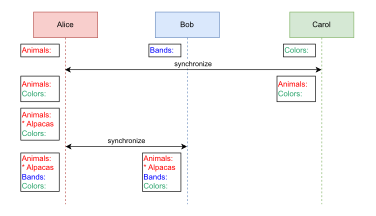
\includegraphics[width=\textwidth]{figures/forward-more-important-than-backward.drawio.pdf}
  \caption{Example for prioritizing forward insertions inspired by Figure 6 in Fugue \protect\cite{2023-weidner-minimizing-interleaving}}
  \label{fig:forward-more-important-than-backward}
\end{figure}

\clearpage

For an insertion in the middle of a text, current editing behavior does not convey whether the insertion semantically belongs to the left side or the right side. Because most text is written in a forward direction, so for left-to-right script from left to right, it is more likely that an insertion in the middle of some text is appending to the left side of the insertion point instead of prepending to the right side of the insertion point. \Cref{fig:forward-more-important-than-backward} exemplifies this. The three replicas \textcolor{red}{Alice}, \textcolor{blue}{Bob} and \textcolor{mygreen}{Carol} independently add three lists to some text. Then, \textcolor{red}{Alice} and \textcolor{mygreen}{Carol} synchronize. Afterwards, \textcolor{red}{Alice} adds \texttt{"\textcolor{red}{*~Alpacas}"} to her list, such that it comes after \texttt{"\textcolor{red}{Animals:}"} and before \texttt{"\textcolor{mygreen}{Colors:}"} but inherently there is no information to which part it belongs. Finally, \textcolor{red}{Alice} and \textcolor{blue}{Bob} synchronize. This separates \texttt{"\textcolor{red}{*~Alpacas}"} and \texttt{"\textcolor{mygreen}{Colors:}"} by the received \texttt{"\textcolor{blue}{Bands:}"}, which may not be wanted. In this example the assumption of the more common forward insertion is correct though. Further improvements to this would need analysis of the language semantics of the text which \Citeauthor*{2023-bauwens-nlp-for-merging} looked into \cite{2023-bauwens-nlp-for-merging}. For the concrete example, a different idea could be to insert \texttt{"\textcolor{blue}{Bands:}"} after \texttt{"\textcolor{mygreen}{Colors:}"} so \texttt{"\textcolor{red}{*~Alpacas}"} stays in place in relation to the text preceding and following it. Unfortunately this would lead to even more unexpected behavior for example when \textcolor{blue}{Bob} and \textcolor{mygreen}{Carol} synchronized before and would order the entries alphabetically because they do not know about the insertion of \texttt{"\textcolor{red}{*~Alpacas}"}. As soon as \textcolor{red}{Alice} would then synchronize with them, the entries would need to be reordered, so that they converge. As the synchronized data is not structured like the example may suggest, but instead consists of arbitrary characters, this reordering could result in sentence reordering or other unwanted results. Another idea could be to prefer the side by the same replica. This has similar issues if concurrent edits are received later and change the effect of that rule.

\section{Fugues Approach to Avoid Text Interleaving} \label{section:challenges-text-interleaving-fugue}

This section shows the proposed solution by Fugue \cite{2023-weidner-minimizing-interleaving} to solve text interleaving. It also gives an example that the proposed \textit{maximally non-interleaving} property can still interleave text when deletions are involved.

\Citeauthor*{2023-weidner-minimizing-interleaving} \cite{2023-weidner-minimizing-interleaving} show that a previous attempt at formalizing a property for non-interleaving by \Citeauthor*{2019-Kleppmann-incorrect-noninterleaving-property} \cite{2019-Kleppmann-incorrect-noninterleaving-property} is incorrect \cite[Section 2.5]{2023-weidner-minimizing-interleaving}. Therefore, they propose their own property which they refer to as \textit{maximally non-interleaving}. It associates every inserted character with the character to its left and right, which they label left and right origin. The property orders the characters by prioritizing keeping the left origin as the previous character because of the common forward insertions and otherwise ordering to preserve the right origin as the following character if possible. Only if both origins are the same, the order is arbitrary but deterministically chosen. Therefore, this property creates a unique order aside from tie-breaking \cite[Section 4.5]{2023-weidner-minimizing-interleaving}.

Fugue refers to an interleaving issue as forward interleaving, when only one character has another character as a left origin, yet the two characters are not consecutive. One example where the Logoot algorithm \cite{2009-weiss-logoot} interleaved characters, which also violates this rule, is concurrently inserting \texttt{"\textcolor{blue}{bread}"} and \texttt{"\textcolor{red}{eggs}"}, producing \texttt{"\textcolor{blue}{b}\textcolor{red}{e}\textcolor{blue}{r}\textcolor{red}{g}\textcolor{blue}{e}\textcolor{red}{g}\textcolor{blue}{a}\textcolor{red}{s}\textcolor{blue}{d}"} \cite[Section 4.4.1]{2019-sun-difference-ot-crdt-2-correctness-complexity}. For example the \texttt{"\textcolor{blue}{r}"} from \texttt{"\textcolor{blue}{bread}"} has the \texttt{"\textcolor{blue}{b}"} as its left origin and no other character has the \texttt{"\textcolor{blue}{b}"} as its left origin but in the result they are not consecutive characters.

\Citeauthor*{2023-weidner-minimizing-interleaving} refer to another problem that many prior algorithms exhibit as backward interleaving. When two insertions have the same left origin but a different right origin, they should be ordered in a way that they are consecutive with their right origins. Although it may seem this is not a common use case, the following is a plausible example \cite[Figure 2]{2023-weidner-minimizing-interleaving}. Starting with the text \texttt{"Shopping"}, \textcolor{red}{Alice} first appends \texttt{"\textcolor{red}{*~apples}"} after \texttt{"Shopping"} and then prepends \texttt{"\textcolor{red}{Fruit:}"} before \texttt{"\textcolor{red}{*~apples}"}. While semantically she is prepending, both inserted texts have \texttt{"Shopping"} as their left origin and different right origins. Concurrently, \textcolor{blue}{Bob} first appends \texttt{"\textcolor{blue}{*~bread}"} after \texttt{"Shopping"} and then prepends \texttt{"\textcolor{blue}{Bakery:}"} before \texttt{"\textcolor{blue}{*~bread}"}. The category insertions by \textcolor{red}{Alice} and \textcolor{blue}{Bob} both have \texttt{"Shopping"} as their left origin but different right origins. Therefore, this should lead to either the outcome of \texttt{"Shopping\textcolor{red}{Fruit:*~apples}\textcolor{blue}{Bakery:*~bread}"} or \texttt{"Shopping\textcolor{blue}{Bakery:*~bread}\textcolor{red}{Fruit:*~apples}"} which only differ in the order of which users text comes first, which is arbitrary. When algorithms exhibit backward interleaving, \texttt{"Shopping\textcolor{blue}{Bakery:}\textcolor{red}{Fruit:}\textcolor{blue}{*~bread}\textcolor{red}{*~apples}"} can be a possible result.
Note that the order of the elements has not changed in relation to each other (e.g. \texttt{"\textcolor{red}{Fruit:}"} comes before \texttt{"\textcolor{red}{*~apples}"} and after \texttt{"Shopping"}) but this still violates the intent of the user.

According to \Citeauthor*{2023-weidner-minimizing-interleaving}, many popular algorithms they looked into exhibit either forward or backward interleaving \cite[Table 1]{2023-weidner-minimizing-interleaving}. A review by \Citeauthor*{2023-sun-critical-examination-fugue-ot} \cite{2023-sun-critical-examination-fugue-ot,2023-sun-critical-examination-fugue-ot-1,2023-sun-critical-examination-fugue-ot-2,2023-sun-critical-examination-fugue-ot-3} that refutes these claims for OT algorithms is addressed in \Cref{chapter:ot}. For Logoot \cite{2009-weiss-logoot} the character-by-character interleaving issue occurs. Further examples are provided in the appendix of the Fugue paper \cite{2023-weidner-minimizing-interleaving}. While the prior \gls{crdt} algorithms YjsMod\footnote{\url{https://github.com/josephg/reference-crdts}} and Sync9\footnote{\url{https://braid.org/sync9}} do not exhibit interleaving \cite[Table 1]{2023-weidner-minimizing-interleaving}, those approaches were not considered here due to the lack of documentation and their intrinsic complexity. \Citeauthor*{2023-weidner-minimizing-interleaving} propose their own algorithms Fugue and FugueMax to solve these problems. They conjecture that Sync9 is semantically equivalent to Fugue and YjsMod is semantically equivalent to FugueMax \cite[Section 6]{2023-weidner-minimizing-interleaving}. They also prove that FugueMax fulfills the \textit{maximally non-interleaving} property \cite[Theorem 9]{2023-weidner-minimizing-interleaving}, prove that the Fugue algorithm is always forward non-interleaving \cite[Lemma 7]{2023-weidner-minimizing-interleaving} and argue that it is also backward non-interleaving when there are not multiple interacting concurrent updates \cite[Section 4.3]{2023-weidner-minimizing-interleaving}.

A counter example that interleaving can also happen for the \textit{maximally non-interleaving} FugueMax algorithm is the following. Starting with the text \texttt{"Shopping"}, \textcolor{red}{Alice} appends \texttt{"\textcolor{red}{*~apples}"} after \texttt{"Shopping"} and then prepends \texttt{"\textcolor{red}{Fruit:}"} before \texttt{"\textcolor{red}{*~apples}"}. Concurrently, \textcolor{blue}{Bob} appends \texttt{"\textcolor{blue}{*~bread}"} after \texttt{"Shopping"}, then deletes and reinserts the \texttt{"\textcolor{blue}{g}"} of \texttt{"Shopping"} and finally prepends \texttt{"\textcolor{blue}{Bakery:}"} before \texttt{"\textcolor{blue}{*~bread}"}. The expected result would be \texttt{"Shoppin\textcolor{blue}{gBakery:*~bread}\textcolor{red}{Fruit:*~apples}"} but the actual result can be \texttt{"Shoppin\textcolor{blue}{gBakery:}\textcolor{red}{Fruit:*~apples}\textcolor{blue}{*~bread}"} when the replicas IDs have a specific order. The code in \Cref{appendix:code-fuguemax-interleaving} verifies this with the reference implementation\footnote{\url{https://github.com/mweidner037/fugue}}. The reason the \textit{maximally non-interleaving} property does not cover this case is that it disregards deletions. This example shows that this simplification is not suitable to ensure non-interleaving.

The basic implementation of Fugue has a linear runtime per character insertion or deletion in relation to the text length (including deleted text) which proved to be too inefficient for larger text given the resulting runtime scales quadratically with the text length. Comparing the results\footnote{\url{https://github.com/mweidner037/fugue/blob/main/results_table.md}} from \Citeauthor*{2023-weidner-minimizing-interleaving} for benchmark B1.1 with benchmark B1.3 indicates, that even the optimized variant in the Fugue paper has quadratic runtime for sequential backward insertions.

\clearpage

\begin{figure}
  \centering
  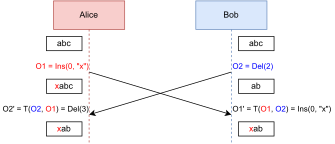
\includegraphics[width=\textwidth]{figures/ot.drawio.pdf}
  \caption{Example for operation transformation with two synchronizing peers based on figure by \Citeauthor*{2024-sun-ot-faq} \cite[Section 1.4 Figure 1]{2024-sun-ot-faq}}
  \label{fig:ot-example}
\end{figure}

\begin{listing}
  \begin{minted}{text}
Tii(Ins[p1,c1], Ins[p2, c2]) {
  if p1 < p2 or (p1 = p2 and u1 > u2)
    return Ins[p1, c1];              
  else
    return Ins[p1+1, c1];
}
\end{minted}
  \caption{Example for transformation function from Sun \cite[Section 2.15]{2024-sun-ot-faq}}
  \label{lst:example-transformation-function}
\end{listing}

\clearpage

\section{OT in Comparison to CRDTs} \label{chapter:ot}

This section explains the differences and similarities between \gls{ot} and \glspl{crdt} and shows that the current \glspl{crdt} runtime complexity is quadratic and current \gls{ot} algorithms are unsuitable for \textit{non-realtime} editing.

While \gls{crdt} papers often claim \glspl{crdt} are superior to \gls{ot}, \glspl{crdt} often miss major relevant parts of the required algorithmic steps which makes them seem potentially simpler and more performant \cite[page 2]{2019-sun-difference-ot-crdt-1-general-transformation-framework}. For example, \glspl{crdt} need to extract the text from their internal state and need to be able to address characters based on their text position as most text editors work that way \cite[Section 5.1, Section 5.2]{2019-sun-difference-ot-crdt-1-general-transformation-framework}. \Glspl{crdt} often miss this conversion step which is a major algorithmic complication that also affects their performance a lot \cite[page 2]{2019-sun-difference-ot-crdt-1-general-transformation-framework}. Note that Fugue also has this issue as it does not describe converting the received operations to character offsets \cite[Algorithm 1]{2023-weidner-minimizing-interleaving}.

\Citeauthor*{2019-sun-difference-ot-crdt-1-general-transformation-framework} also show that both approaches are more similar than often presented \cite[Section 4.1 Table 1]{2019-sun-difference-ot-crdt-1-general-transformation-framework}. While \glspl{ot} have position based operations directly on the character sequence that are then transformed by concurrent operations, \glspl{crdt} have identifier based operations on an internal object sequence, that are converted to the position based character sequence after the operations have been applied.

\gls{ot} based algorithms consist of a control algorithm and a transformation function \cite{2024-sun-ot-faq}. The control algorithm is generic, and the transformation function is application specific. For example for plain text editing there could be two operations, Insert(index, character) and Delete(index). The transformation function $T(O_2, O_1)$ transforms $O_2$ against $O_1$. This produces the operation that needs to be applied after $O_1$ if they were concurrent before. \Cref{fig:ot-example} shows an example where the positions of the concurrent operations are transformed when receiving them and therefore result in the same text at both peers. In that example the transformation function could be defined as shown in \Cref{lst:example-transformation-function} for transforming two insert operations \cite[Section 2.15]{2024-sun-ot-faq}. If a concurrent insertion happened at a position after the current insertion it does not need to be transformed. If a concurrent insertion happened at a position before the current insertion it needs to be offset by one. For equal positions, tie breaking using the replica identifier is required.

The control algorithms decide in which order operations need to be transformed to achieve the desired outcome \cite[Section 2.2]{2024-sun-ot-faq}. Depending on the control algorithm, the transformation function needs to fulfill different properties to ensure correctness \cite[Section 2.20]{2024-sun-ot-faq}. Also, some control algorithms are able to handle undo, some can undo arbitrary actions out of order, while some cannot \cite[Section 2.12]{2024-sun-ot-faq}.

Transformation functions need to be defined for all possible combinations of operations. This means $N^2$ such functions are needed for $N$ possible operations. An alternative proposed by \Citeauthor*{2019-sun-difference-ot-crdt-3-building-real-world-applications} is POT+COA (Primitive Operation
Transformation plus Complex Operation Adaptation). It consists of having some primitive operations for which transformation functions are defined, and then complex application operations are converted to these primitive operations \cite[Section 2.1.3]{2019-sun-difference-ot-crdt-3-building-real-world-applications}.

OT based algorithms can be integrated into existing editors with little change of the editors source code as OT is operation and concurrency-centric. The algorithm can just apply the received and transformed operations to the local editor and send local operations to other peers. \Citeauthor*{2019-sun-difference-ot-crdt-3-building-real-world-applications} refer to this as Transparent Adaptation (TA) \cite[Section 2.1.2]{2019-sun-difference-ot-crdt-3-building-real-world-applications}.

According to \Citeauthor*{2019-sun-difference-ot-crdt-1-general-transformation-framework}, \gls{ot} uses a concurrency-centric and direct transformation approach and \gls{crdt} uses a content-centric and indirect transformation approach \cite[Section 1]{2019-sun-difference-ot-crdt-1-general-transformation-framework}. This has an important consequence for the time and space complexity. The time and space complexity of \gls{ot} for \textit{realtime} editing depends on the number of concurrent operations which are usually small in realtime text editing while the time and space complexity of \gls{crdt} depends on the length of the text or even the length of the text including all deleted content which are usually a lot larger \cite[Section 5.3]{2019-sun-difference-ot-crdt-1-general-transformation-framework}. The time complexity for prior \gls{ot} based algorithms is at least $O(c)$ per remote operation \cite[Section 3.1.4]{2019-sun-difference-ot-crdt-2-correctness-complexity}. This means quadratic runtime complexity in relation to the operation count for handling some count of operations, which is unusable for \textit{non-realtime} editing because there can be many concurrent operations. It is important to mention that the time complexity class is relevant. For example, $O(\log(\text{text-length-including-deletions}))$ runtime complexity can be equally acceptable to $O(\text{concurrent-operations})$ runtime complexity because $O(\log(n))$ is growing quite slowly even for extremely large inputs. Prior research of \glspl{crdt} mostly managed a linear time complexity or worse except of a paper by \Citeauthor*{2016-briot-logn-optimization} which optimizes an \gls{rga} adaptation to $O(\log(n))$ per operation similarly to us \cite[Table 4]{2019-sun-difference-ot-crdt-2-correctness-complexity}. However, \Citeauthor*{2016-briot-logn-optimization} have not gone into the analysis of performance edge cases prohibiting us from drawing a fair comparison. Additionally, it is unclear whether they include the conversion of remote operations to character positions. Furthermore, as the algorithm is based on \gls{rga}, it exhibits interleaving \cite[Table 1]{2023-weidner-minimizing-interleaving}.

While \glspl{crdt} often seem to be simple and easy to understand, the fundamental concurrency issues which are inherent to unconstrained co-editing also exist there and mixing content and concurrency creates new difficulties with handling them \cite[Section~4]{2019-sun-difference-ot-crdt-2-correctness-complexity}.

\include{chapters/background}
\IMRADlabel{methods}
\chapter{Implementation of Fugue Algorithm} \label{section:implementation}

This chapter first lists the requirements for an implementation of the Fugue algorithm in \Cref{section:implementation-requirements}. \Cref{section:implementation-browser} gives insights into our editor implementation in the browser and our \gls{p2p} functionality and \Cref{sec:synchronization} explains how our synchronization works and is optimized. \Cref{sec:property-tests} introduces our use of property tests to ensure convergence of our implementation and argues that extensive use of assertions for invariants aids in finding the root cause of test failures. Finally, \Cref{section:implementation-issues-algorithmic-description} reveals some small issues in the algorithmic description in the Fugue paper \cite{2023-weidner-minimizing-interleaving}.

The source code is available at:\\
\url{https://github.com/mohe2015/bachelor-thesis-collaborative-text-editing}

\section{Required Implementation Functionality} \label{section:implementation-requirements}

Based on the Fugue paper \cite{2023-weidner-minimizing-interleaving} and our explanation of the Fugue algorithm in the last chapter, an implementation needs to provide the following functionality:

It needs to provide an interface to a tree with left and right children, possibly multiple children on each side but usually only one on one side. It requires fast retrieval of a node based on an index in the non-deleted node traversal and fast retrieval of an index in the non-deleted node traversal based on the node. Additionally, it requires fast retrieval of a node based on its ID. For initial loading it also needs to be able to traverse the whole tree in order. Furthermore, inserting nodes to the right and left of other nodes needs to be efficient with the special case of multiple left or right children.

In practice, trees usually contain many deep right descendants because of consecutive character insertions \cite[Figure 5]{2023-weidner-minimizing-interleaving}, so this is a case that should be heavily optimized.

\begin{listing}
  \begin{minted}{scala}
val schema = Schema(SchemaSpec(orderedmap.from(StringDictionary(
  ("text", NodeSpec()),
  ("doc",
    NodeSpec()
      .setContent("text*")
      .setMarks("")
      .setCode(true)
      .setDefining(true)
      .setParseDOM(
        js.Array(TagParseRule("pre").setPreserveWhitespace(full)))
      .setToDOM(_ => Array("pre", 0)))))))
val hardBreakCommand: Command = (state, dispatch, view) => {
  dispatch.get(state.tr.insertText("\n"))
  true
}
val editorStateConfig = EditorStateConfig().setSchema(schema)
  .setPluginsVarargs(keymap(StringDictionary(("Enter", hardBreakCommand))))
\end{minted}
  \caption{Code excerpt of ProseMirror schema setup}
  \label{lst:prosemirror-schema}
\end{listing}



\section{Browser Implementation of Text Editor} \label{section:implementation-browser}

To properly use text editing algorithms an editor is required, so we implement an interface to ProseMirror\footnote{\url{https://prosemirror.net/}} and transpile Scala to JavaScript using Scala.js\footnote{\url{https://www.scala-js.org/}} to be able to use our implementation on the web.

By default, ProseMirror creates newlines using \texttt{<br/>}~tags and paragraphs using \texttt{<p>}~tags. This makes it complicated to convert between the ProseMirror document offset and the text offset. Therefore, we configured ProseMirror to only support plaintext and use \texttt{\textbackslash n} for newlines and configured the browser to render \texttt{\textbackslash n} as newlines (which does not work by default) as shown in \Cref{lst:prosemirror-schema}.

We also implemented a demo using WebRTC\footnote{\url{https://webrtc.org/}} to collaboratively edit a text. It keeps the full history on all connected peers, so it is not possible to permanently delete anything. This is the reason for not implementing persistence, see \Cref{sec:data-privacy-issues}.

\section{Synchronization of Changes} \label{sec:synchronization}

The changes are synchronized using causal broadcast as in the Fugue paper \cite{2023-weidner-minimizing-interleaving}. The events are ordered using vector clocks \cite{1988-mattern-vector-clock,1988-fidge-vector-clock}. Only change synchronization updates the vector clock. Therefore, the clock does not need to be updated while working offline, and the changes can be sent in one batch which is more efficient. Instead of creating a message per character insertion or deletion, consecutive deletions and insertions that have the same causality are combined to optimize memory usage.

\section{Testing Using Property Tests}\label{sec:property-tests}

Property tests are a core part of testing \glspl{rdt} as the existence of numerous edge cases make unit testing infeasible. The tests run both on the internal data structure, with an interface for inserting and deleting characters at indices, and on the local web application as a Playwright\footnote{\url{https://playwright.dev/java/}} test.

The property tests run using ScalaCheck\footnote{\url{https://scalacheck.org/}} and specifically its stateful testing support\footnote{\url{https://github.com/typelevel/scalacheck/blob/main/doc/UserGuide.md\#stateful-testing}} using \texttt{Commands}\footnote{\label{footnote:commands}\url{https://github.com/typelevel/scalacheck/blob/main/core/shared/src/main/scala/org/scalacheck/commands/Commands.scala}}. ScalaCheck \texttt{Commands} store a system under test and a state that is compared to the system under test. Possible actions are defined by implementing the \texttt{Command}\footref{footnote:commands} trait. The trait has several methods for pre conditions, post conditions, running the action and calculating the next state. ScalaCheck generates \texttt{Command}s and their contents using Generators, e.g. \texttt{Gen.chooseNum(0, Int.MaxValue)} which are then run by ScalaCheck against the system under test and if failures occur it tries to simplify the failure case.

Our property tests randomly create replicas, synchronize replicas, insert text at a replica or delete text at a replica. Then, they check whether replicas have the same text after they synchronized. Unfortunately it is not easily possible to check \textit{what} the expected text would be as that would need more or less a reimplementation of the synchronization logic, see \Cref{section:future-work-correctness}. We also have property tests that check that local operations match the same operations on a \texttt{String}.

While trying out new approaches, implementation mistakes are likely, particularly when more complicated approaches have lots of edge cases. It is really laborious to find the root cause for every test failure to fix edge cases, especially for property tests that do not always produce the smallest possible test case. It helps significantly to add lots of assertions into the code that not only check local conditions like traditional uses of assertions but also check global invariants. Some examples of such assertions are ensuring that parent and child references are symmetric to each other and that insertions and deletions correctly update the positions of all characters. These assertions strongly affect the performance, so they need to be disabled for production use.

Ideally, invariant assertions would be automatically checked after every object creation and modification, but that is not easily possible with Scala. Therefore, they were added manually at relevant places. The tests also detect the bugs without these invariant assertions. The failure then happens at a later time in execution, which complicates finding the root cause, but does not decrease the reliability.

\section{Issues in the Algorithmic Description} \label{section:implementation-issues-algorithmic-description}

While working on our implementation, we found that the algorithmic description \cite[Algorithm~1]{2023-weidner-minimizing-interleaving} is, for the most part, satisfactory. However, it contains one large issue. While the Fugue paper includes the conversion from character offsets to their internal representation, it misses the reverse direction \cite[Algorithm~1]{2023-weidner-minimizing-interleaving}. Received operations also need to be converted to the index to update the local text editor. Therefore, we extended the algorithmic description with that. This is not just relevant for implementation but also for optimization, which we address in the next chapter. It means that further functionality is required, that can map a node ID to the position in the tree traversal of visible nodes, which is the visible text. The remaining issues were only minor or instances of suboptimal specification.

First, the ID type \cite[Algorithm~1]{2023-weidner-minimizing-interleaving} can always be \texttt{null}. As this can only be the case for the root node, we moved this case to the places where the root node could potentially be used. There are some places where this could \textit{not} be the case, e.g. remote insertions can not send the root node as the root node is always locally created.

Second, in line 10 of the description \cite[Algorithm~1]{2023-weidner-minimizing-interleaving}, root is initialized with a value that is invalid according to their specification because the side can only be \texttt{L} or \texttt{R} but never \texttt{null} according to the types. Our implementation arbitrarily chooses the root node to be on the right side to simplify checks at other places in the code. An alternative would be to use an enumeration for the node and not have an ID, value, side and parent for the root node at all.

Third, each node does not necessarily need to store the ID of its parent and children \cite[Algorithm~1]{2023-weidner-minimizing-interleaving}. It could also store a reference directly to them.

Lastly, the node after \texttt{leftOrigin} in line 24 \cite[Algorithm~1]{2023-weidner-minimizing-interleaving} can be retrieved as the leftmost descendant of the first right child of the \texttt{leftOrigin}. The leftmost descendant is the node that is reached by repeatedly descending into the leftmost child until there are no left children. This is logical as the next node must be in the right subtree and there the first node is the leftmost node. Depending on the implementation that may be faster or easier.

\include{chapters/optimization}
\IMRADlabel{results}
\include{chapters/evaluation}
\IMRADlabel{discussion}
\include{chapters/future-work}
\chapter{Conclusion} \label{chapter:conclusion}

This thesis shows that efficient collaborative plain text editing in a decentralized and \textit{non-realtime} setting while preserving user intentions is possible. The optimization to logarithmic runtime per operation in relation to the text length ensures that this is also efficient for extremely large text. This thesis also shows that prior benchmarks do not measure asymptotic complexity and do not cover all algorithmic performance edge cases and proposes to include both in future benchmarks. This is especially an issue in decentralized networks, as there is only limited control over all messages and peers can send you messages with malicious content that triggers these edge cases.

The WebRTC implementation shows a practical example of text editing in \gls{p2p} networks and allows easy experimentation.

\Cref{section:challenges-text-interleaving} shows that interleaving for the \textit{maximally non-interleaving} property \cite{2023-weidner-minimizing-interleaving} is indeed possible when deletions are involved. Therefore, a more accurate property should be researched to ensure non-interleaving.

Significant parts that are common in text editing are still missing, the largest being rich text support. Rich text support likely leads to further implementation and optimization challenges, and it is not clear whether these are solvable while preserving the same asymptotic complexity in all cases. Additionally, the preservation of user intentions of formatting actions likely has similar challenges as ensuring non-interleaving has. The interaction of rich text and being able to undo arbitrary actions likely also poses further challenges.

While testing whether the algorithm converges is comparably simple, testing intent preservation and non-interleaving without reimplementing the algorithm in the test is challenging. As testing is a critical part to ensure correctness, more focus needs to be put on testing text editing algorithms.
\chapter*{Acknowledgments}
I would like to thank everyone who reviewed drafts of this thesis. I would also like to thank my human and non-human rubber ducks for their help in debugging my code.

\printglossary[type=\acronymtype]

\printbibliography

\appendix

\RedeclareSectionCommand[beforeskip=0pt]{chapter}
\chapter{Appendix}
\label{appendix:appendix}
\section{CPU Profile for Simple Algorithm with Sequential Insertions}
\label{appendix:simple-sequential-inserts-cpu}
\includegraphics[width=\textwidth,height=\textheight,keepaspectratio]{../text-rdt/target/pdfs/simple-sequential-inserts-cpu.pdf}
\section{CPU Profile for Batching Algorithm with Sequential Insertions}
\label{appendix:complex-sequential-inserts-cpu}
\includegraphics[width=\textwidth,height=\textheight,keepaspectratio]{../text-rdt/target/pdfs/complex-sequential-inserts-cpu.pdf}
\section{Allocation Profile for Batching Algorithm with Sequential Insertions}
\label{appendix:complex-sequential-inserts-alloc}
\includegraphics[width=\textwidth,height=\textheight,keepaspectratio]{../text-rdt/target/pdfs/complex-sequential-inserts-alloc.pdf}
\section{CPU Profile for Batching Algorithm with Real World Dataset}
\label{appendix:complex-real-world-cpu}
\includegraphics[width=\textwidth,height=\textheight,keepaspectratio]{../text-rdt/target/pdfs/complex-real-world-cpu.pdf}
\section{CPU Profile for Simple AVL Algorithm with Real World Dataset}
\label{appendix:simpleavl-real-world-cpu}
\includegraphics[width=\textwidth,height=\textheight,keepaspectratio]{../text-rdt/target/pdfs/simpleavl-real-world-cpu.pdf}
\section{Allocation Profile for Simple AVL Algorithm with Real World Dataset}
\label{appendix:simpleavl-real-world-alloc}
\includegraphics[width=\textwidth,height=\textheight,keepaspectratio]{../text-rdt/target/pdfs/simpleavl-real-world-alloc.pdf}

\clearpage

\section{Code Showing FugueMax Is Interleaving}
\label{appendix:code-fuguemax-interleaving}
\begin{minted}{typescript}
let rng = seedrandom("42");
let docA = new CRuntime({
  debugReplicaID: ReplicaIDs.pseudoRandom(rng),
});
let ctextA = docA.registerCollab(
  "text",
  (init) => new FugueMaxSimple(init)
);
let docB = new CRuntime({
  debugReplicaID: ReplicaIDs.pseudoRandom(rng),
});
let ctextB = docB.registerCollab(
  "text",
  (init) => new FugueMaxSimple(init)
);
let messageA: Uint8Array = null!
docA.on("Send", (e) => {
  messageA = e.message
})
let messageB: Uint8Array = null!
docB.on("Send", (e) => {
  messageB = e.message
})
docA.transact(() => {
  ctextA.insert(0, 'S')
  ctextA.insert(1, 'h')
  ctextA.insert(2, 'o')
  ctextA.insert(3, 'p')
  ctextA.insert(4, 'p')
  ctextA.insert(5, 'i')
  ctextA.insert(6, 'n')
  ctextA.insert(7, 'g')
})
docB.receive(messageA)
docB.transact(() => {
  ctextB.insert(8, '*')
  ctextB.insert(9, 'b')
  ctextB.insert(10, 'r')
  ctextB.insert(11, 'e')
  ctextB.insert(12, 'a')
  ctextB.insert(13, 'd')
  ctextB.delete(7)
  ctextB.insert(7, 'g')
  ctextB.insert(8, 'B')
  ctextB.insert(9, 'a')
  ctextB.insert(10, 'k')
  ctextB.insert(11, 'e')
  ctextB.insert(12, 'r')
  ctextB.insert(13, 'y')
  ctextB.insert(14, ':')
})
docA.transact(() => {
  ctextA.insert(8, '*')
  ctextA.insert(9, 'a')
  ctextA.insert(10, 'p')
  ctextA.insert(11, 'p')
  ctextA.insert(12, 'l')
  ctextA.insert(13, 'e')
  ctextA.insert(14, 's')
  ctextA.insert(8, 'F')
  ctextA.insert(9, 'r')
  ctextA.insert(10, 'u')
  ctextA.insert(11, 'i')
  ctextA.insert(12, 't')
  ctextA.insert(13, ':')
})
docB.receive(messageA)
docA.receive(messageB)
console.log([...ctextA.values()].join(""))
console.log([...ctextB.values()].join(""))
\end{minted}

\end{document}
